\documentclass[aps,prd,preprint,nofootinbib,superscriptaddress]{revtex4-2}

\usepackage[T1]{fontenc}
\usepackage[utf8]{inputenc}
\usepackage{amsmath,amssymb,mathtools}
\usepackage{bm}
\usepackage{booktabs}
\usepackage{graphicx}
\usepackage{xcolor}
\usepackage[colorlinks=true,linkcolor=blue,citecolor=blue,urlcolor=blue]{hyperref}

\newcommand{\ii}{\mathrm{i}}
\newcommand{\Ds}{D_s}
\newcommand{\Dst}{D_s^*}
\newcommand{\Dsone}{D_{s1}}
\newcommand{\Bs}{B_s}
\newcommand{\Bst}{B_s^*}
\newcommand{\Bsone}{B_{s1}}
\newcommand{\GeV}{\mathrm{GeV}}
\newcommand{\MeV}{\mathrm{MeV}}
\newcommand{\keV}{\mathrm{keV}}
\newcommand{\qqbar}{\langle\bar q q\rangle}
\newcommand{\ssbar}{\langle\bar s s\rangle}

\begin{document}

\title{Radiative transitions of strange heavy axial mesons in light-cone QCD sum rules}

\author{S. Bilmis}
\affiliation{Department of Physics, Middle East Technical University, Ankara, Turkey}
\author{T. M. Aliev}
\affiliation{Department of Physics, Middle East Technical University, Ankara, Turkey}
\author{M. Savci}
\affiliation{Department of Physics, Middle East Technical University, Ankara, Turkey}

\date{\today}

\begin{abstract}
We study the radiative transitions
$\Dsone(2460)\to \Ds\gamma$, $\Dsone(2536)\to \Ds\gamma$, and
$\Bsone(5830)\to \Bs\gamma$ in light-cone QCD sum rules.  The calculation keeps
strange-quark-mass terms, hard photon emission, and two- and three-particle
photon distribution-amplitude contributions.  With the lattice-normalized
photon distribution amplitude we obtain
$\Gamma[\Dsone(2460)\to\Ds\gamma]=16.1^{+4.4}_{-3.7}~\keV$ and
$\Gamma[\Dsone(2536)\to\Ds\gamma]=0.50^{+0.60}_{-0.38}~\keV$.
The strong suppression of the latter mode follows from destructive interference
between the two physical-current components.
\end{abstract}

\maketitle

\section{Introduction}

The spectroscopy of positive-parity strange heavy mesons remains a useful
testing ground for the interplay between heavy-quark symmetry, light-quark
dynamics, and nearby hadronic thresholds.  The charm-strange states
$\Dsone(2460)$ and $\Dsone(2536)$ are especially interesting.  The lower state
is very narrow and has observed radiative decay modes, whereas the upper state
is seen clearly in hadronic channels but its radiative transition to
$\Ds\gamma$ has not been observed with a comparable significance
\cite{BaBar:2006eep,BaBar:2011zpy,Belle:2007hue}.  In the bottom-strange
sector the state $\Bsone(5830)$ has been established in hadronic spectroscopy
\cite{CMS:2018qdl}, while direct radiative information is still absent.

Radiative widths of these mesons have been considered in quark models,
relativistic quark models, effective approaches, and phenomenological analyses
\cite{Godfrey:2005ww,Goity:2000dk,Radford:2009bs,Green:2016occ,Chen:2020ejk,
Korner:1992pz,Li:2021qgz,Godfrey:2016nwn,Lu:2016bbk,Bondar:2023mua,
Bondar:2025smw}.  A recent observation by Bondar and Milstein is particularly
relevant for the present work: the smallness of
$\Dsone(2536)\to\Ds\gamma$ can be understood as a cancellation between the two
spin components of the physical axial state \cite{Bondar:2023mua,
Bondar:2025smw}.  One of our aims is to examine the same mechanism in a
light-cone QCD sum-rule (LCSR) calculation.

The LCSR method expresses the correlation function near the light cone in
terms of photon distribution amplitudes (DAs) and hadronic decay constants
\cite{Shifman:1978bx,Braun:1997kw,Ball:2002ps}.  It is well suited for
exclusive radiative transitions because it keeps the hard photon emission from
quark lines and the long-distance photon emission encoded in photon DAs in a
single framework.  In the present analysis we include both quark-line hard
emission terms, the two-particle photon DAs, and the three-particle photon-DA
terms induced by the background-gluon insertion in the quark propagator.  We
also keep the terms proportional to the strange-quark mass.

The paper is organized as follows.  In Sec.~\ref{sec:framework} we define the
currents, the radiative form factor, and the LCSR correlation function.  The
sum-rule derivation and the physical-current normalization are summarized in
Sec.~\ref{sec:sumrule}.  Section~\ref{sec:numerics} contains the input
parameters, Borel-window discussion, numerical results, comparison with other
studies, and experimental interpretation.  We conclude in Sec.~\ref{sec:concl}.

\section{Theoretical framework}
\label{sec:framework}

We consider the transition of an axial strange heavy meson with momentum
$P=p+q$ into a pseudoscalar strange heavy meson with momentum $p$ and a real
photon with momentum $q$.  The pseudoscalar interpolating current is
\begin{equation}
  J_5=\bar s\,\ii\gamma_5 Q, \qquad Q=c,b .
\end{equation}
For the axial channel we use the two basis currents
\begin{align}
  J^A_\mu &= \bar s\gamma_\mu\gamma_5 Q, \\
  J^B_\mu &= \frac{\ii}{m_Q+m_s}\,
  \bar s\sigma_{\mu\alpha}P^\alpha\gamma_5 Q ,
  \label{eq:basis-currents}
\end{align}
where $P^\alpha$ is the momentum of the initial axial meson.  The physical
currents are written as
\begin{align}
  J_{1\mu} &= \sin\theta\,J^A_\mu+\cos\theta\,J^B_\mu,\\
  J_{2\mu} &= \cos\theta\,J^A_\mu-\sin\theta\,J^B_\mu .
  \label{eq:physical-currents}
\end{align}
Unless stated otherwise we use $\theta=35.3^\circ$ and include the interval
$25^\circ\leq\theta\leq45^\circ$ as a systematic scan.

The radiative matrix element is parametrized by a single gauge-invariant
electric-dipole form factor:
\begin{equation}
  \langle P(p)\gamma(q,\varepsilon)|A(P,\eta)\rangle
  =
  eG\left[(\eta\cdot\varepsilon^*)(p\cdot q)
  -(\eta\cdot q)(p\cdot\varepsilon^*)\right].
  \label{eq:e1}
\end{equation}
The corresponding width is
\begin{equation}
  \Gamma(A\to P\gamma)
  =
  \frac{\alpha_{\rm em}}{3}\,G^2
  \left(\frac{m_A^2-m_P^2}{2m_A}\right)^3 .
  \label{eq:width}
\end{equation}

\section{Light-cone sum rule}
\label{sec:sumrule}

The starting point is the vacuum-to-photon correlation function
\begin{equation}
  \Pi_\mu(p,q)=\ii\int d^4x\,e^{\ii p\cdot x}
  \langle\gamma(q,\varepsilon)|
  T\{\bar s(x)\Gamma_\mu Q(x)\,\bar Q(0)\ii\gamma_5 s(0)\}
  |0\rangle ,
  \label{eq:corr}
\end{equation}
where $\Gamma_\mu=\gamma_\mu\gamma_5$ or
$\Gamma_\mu=\ii\sigma_{\mu\alpha}P^\alpha\gamma_5/(m_Q+m_s)$.  We project the
correlator onto
\begin{equation}
  (p\cdot q)\varepsilon_\mu^*-(p\cdot\varepsilon^*)q_\mu,
  \label{eq:projector}
\end{equation}
which matches the structure in Eq.~\eqref{eq:e1}.

On the hadronic side, isolating the ground-state double pole gives
\begin{equation}
  \Pi_\mu^{\rm had}=
  \frac{m_P^2 f_P}{m_Q+m_s}\,
  \frac{m_A f_A^{(i)}G_i}
  {(m_A^2-P^2)(m_P^2-p^2)}
  \left[(p\cdot q)\varepsilon_\mu^*
  -(p\cdot\varepsilon^*)q_\mu\right]+\cdots ,
  \label{eq:hadronic}
\end{equation}
where $i=A,B$ for the basis currents and the ellipsis denotes higher states
and continuum contributions.

The QCD side is obtained by expanding near the light cone in the external
electromagnetic field.  We use the quark propagators in the external photon
and gluon background.  For the heavy-quark line the relevant terms are
\begin{align}
  S_Q(k) &=
  \frac{\not k+m_Q}{m_Q^2-k^2}
  -e_Q\int_0^1du
  \left[
  \frac{\not k+m_Q}{2(m_Q^2-k^2)^2}
  F^{\mu\nu}(ux)\sigma_{\mu\nu}
  +\frac{u x_\mu F^{\mu\nu}(ux)\gamma_\nu}{m_Q^2-k^2}
  \right]
  \notag\\
  &\quad
  -g_s\int_0^1du
  \left[
  \frac{\not k+m_Q}{2(m_Q^2-k^2)^2}
  G^{\mu\nu}(ux)\sigma_{\mu\nu}
  +\frac{u x_\mu G^{\mu\nu}(ux)\gamma_\nu}{m_Q^2-k^2}
  \right]+\cdots .
  \label{eq:heavy-prop}
\end{align}
The light-quark propagator is used consistently in the same external-field
expansion.  Ordinary vacuum-condensate terms are not inserted as independent
three-point contributions in the photon LCSR.  Instead, the long-distance
photon emission is described by photon matrix elements such as
$\langle\gamma|\bar s\sigma_{\mu\nu}s|0\rangle$, whose normalization contains
the susceptibility combination $\chi_s\ssbar$ or, equivalently, the modern
lattice normalization $f_{\gamma,s}^{\perp}$.  This convention is distinct
from the local two-point sum rules for the residues, where the usual SVZ
condensates enter the OPE.

After the double Borel transformation in $p^2$ and $P^2$ and continuum
subtraction, the basis-current form factors are denoted by $G_A$ and $G_B$.
The physical charm-strange couplings are then formed as
\begin{align}
  G_{2460} &=
  \frac{\sin\theta\,f_A\,G_A+\cos\theta\,f_B\,G_B}{f_1},\\
  G_{2536} &=
  \frac{\cos\theta\,f_A\,G_A-\sin\theta\,f_B\,G_B}{f_2}.
  \label{eq:physical-form-factors}
\end{align}
Here $f_1$ and $f_2$ are the residues of the mixed physical currents in
Eq.~\eqref{eq:physical-currents}.  We use a Stage-3 residue normalization in
which $f_1=0.345\pm0.017~\GeV$ is used as the working anchor and the same
two-point overlap model gives $f_2\simeq0.38~\GeV$.  As a check of the basis
normalization, the pure axial-current limit is compared with the QCD sum-rule
result of Ref.~\cite{Wang:2015mxa}.  For the bottom-strange channel we use the
Pullin--Zwicky decay-constant scenario
$f_{\Bsone}=0.305\pm0.027~\GeV$ and
$f_{\Bsone}^{T}=0.285\pm0.027~\GeV$ \cite{Pullin:2021ebn}.

\section{Numerical analysis}
\label{sec:numerics}

\subsection{Input parameters and working windows}

The main numerical inputs are collected in Table~\ref{tab:inputs}.  Masses and
quark masses are taken from the Particle Data Group \cite{ParticleDataGroup:2024cfk}.
The pseudoscalar decay constants are taken from the lattice averages summarized
by FLAG \cite{FlavourLatticeAveragingGroupFLAG:2024oxs}.  The photon DAs are
those of Ball, Braun and Kivel \cite{Ball:2002ps}.  We compare the older
magnetic-susceptibility input \cite{Rohrwild:2007yt} with the recent lattice
normalization of the leading-twist photon DA \cite{Bacchio:2024pij}; the
lattice-normalized scenario is used as our preferred result.

\begin{table}[t]
\caption{Main input parameters.  Photon-DA normalizations are quoted at
$\mu=1~\GeV$.}
\label{tab:inputs}
\begin{ruledtabular}
\begin{tabular}{lll}
Quantity & Value & Comment \\
\hline
$m_c,m_b,m_s$ & $1.27(2),\,4.18(3),\,0.093(11)~\GeV$ & $\overline{\rm MS}$ inputs \\
$M_{2460},M_{2536},m_{\Ds}$ & $2.4595,\,2.53511,\,1.96835~\GeV$ & PDG \\
$M_{5830},m_{\Bs}$ & $5.82870,\,5.36692~\GeV$ & PDG/CMS \\
$f_{\Ds},f_{\Bs}$ & $0.2499,\,0.2303~\GeV$ & FLAG/lattice context \\
$f_1,f_2$ & $0.345(17),\,\simeq0.38~\GeV$ & charm mixed-current residues \\
$f_{\Bsone},f_{\Bsone}^{T}$ & $0.305(27),\,0.285(27)~\GeV$ & bottom PZ scenario \\
$\chi_s(1~\GeV)$ & $+3.15(30)~\GeV^{-2}$ & legacy photon input \\
$f_{\gamma,s}^{\perp}(1~\GeV)$ & $-55.1(1.9)~\MeV$ & preferred photon input \\
\end{tabular}
\end{ruledtabular}
\end{table}

The Borel windows are chosen by requiring a stable prediction under changes of
$M^2$ and the continuum threshold while avoiding regions where continuum
contributions or higher-dimensional terms dominate.  For the charm-strange
case we use $3~\GeV^2\leq M^2\leq6~\GeV^2$ and
$2.50~\GeV\leq\sqrt{s_0}\leq2.60~\GeV$.  For the bottom-strange case we use
$8~\GeV^2\leq M^2\leq14~\GeV^2$.  The representative stability plots are shown
in Fig.~\ref{fig:stability}.

\begin{figure}[t]
\centering
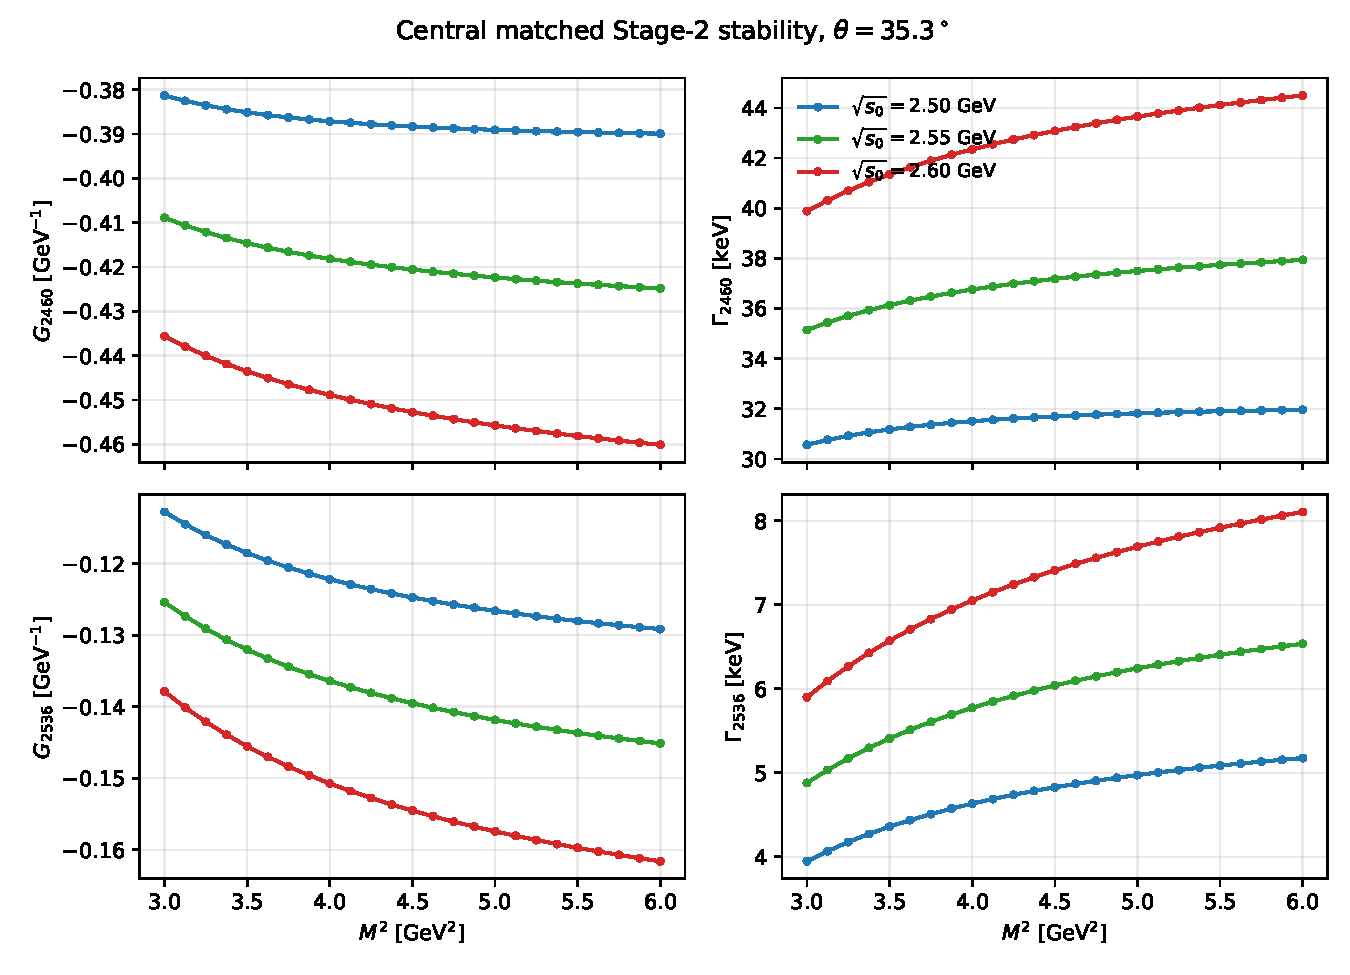
\includegraphics[width=0.47\textwidth]{../outputs/stage2_stability_central.pdf}
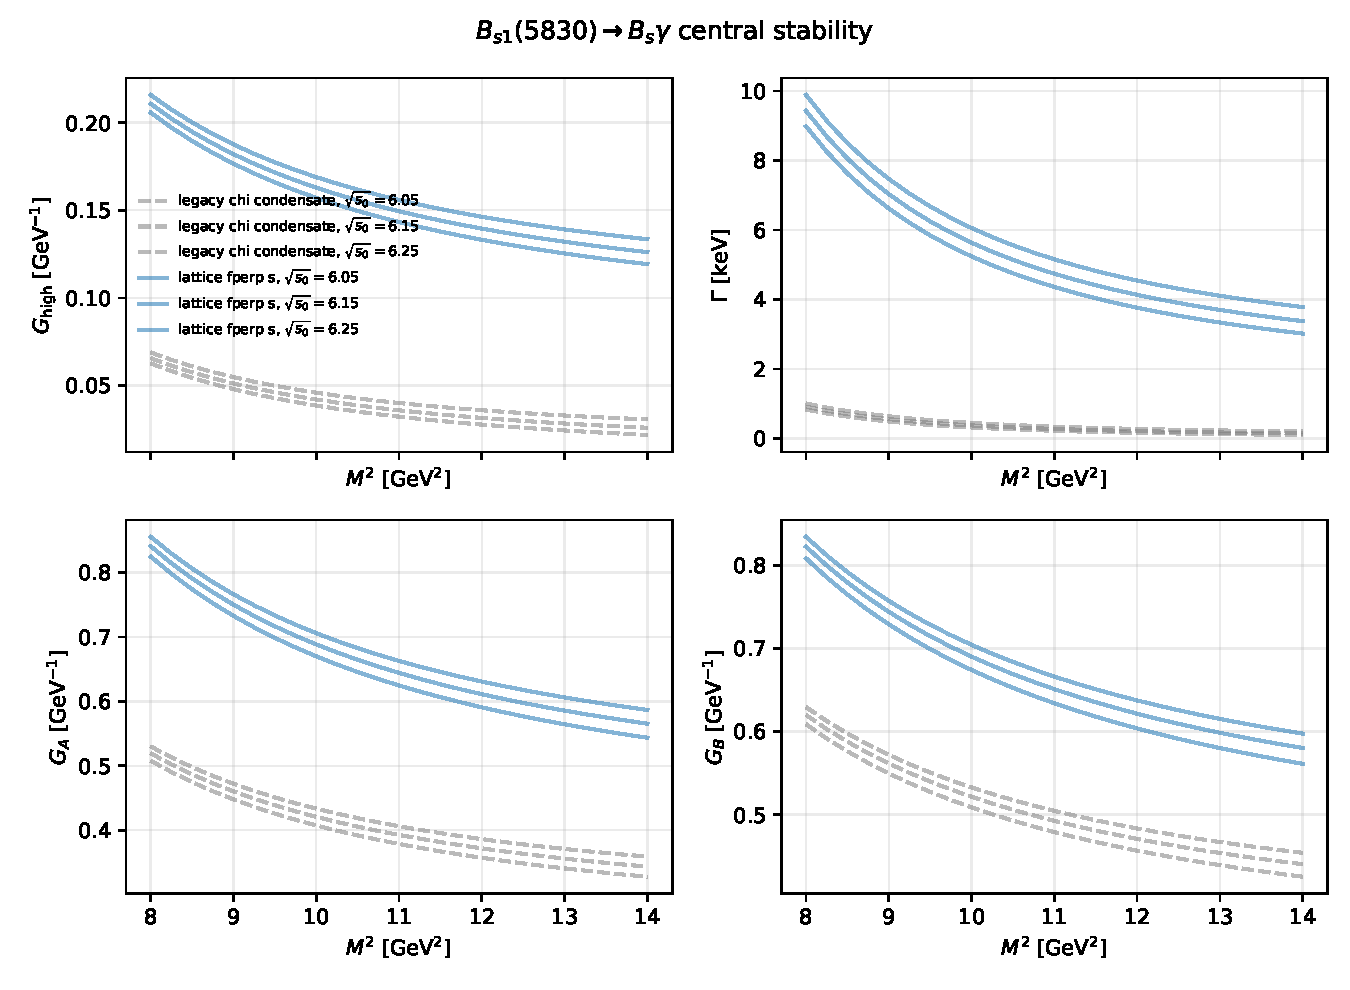
\includegraphics[width=0.47\textwidth]{../outputs/bs1_5830_stability.pdf}
\caption{Representative Borel and continuum-threshold stability checks for
the charm-strange and bottom-strange channels.}
\label{fig:stability}
\end{figure}

\subsection{Results and uncertainties}

The final form factors and widths are listed in Table~\ref{tab:results}.  We
quote medians and 16--84 percentile intervals.  This is preferable to a
Gaussian fit for cancellation-sensitive channels, because the distributions of
$\Dsone(2536)$ and $\Bsone(5830)$ are visibly non-Gaussian near zero.

\begin{widetext}
\begin{table}[t]
\caption{Final form-factor and width predictions.  The lattice photon input is
our preferred normalization.}
\label{tab:results}
\scriptsize
\begin{ruledtabular}
\begin{tabular}{llllcc}
Sector & Decay & Photon input & Normalization & $G~(\GeV^{-1})$ & $\Gamma~(\keV)$\\
\hline
$D_s$ & $\Dsone(2460)\to\Ds\gamma$ & legacy $\chi_s$ & $f_1=0.344[0.329,0.363]$
& $-0.424[-0.484,-0.360]$ & $37.7^{+11.5}_{-10.5}$\\
$D_s$ & $\Dsone(2536)\to\Ds\gamma$ & legacy $\chi_s$ & $f_2=0.380[0.339,0.423]$
& $+0.0118[+0.0014,+0.0233]$ & $0.045^{+0.124}_{-0.040}$\\
$D_s$ & $\Dsone(2460)\to\Ds\gamma$ & lattice $f_{\gamma,s}^{\perp}$ & $f_1=0.345[0.330,0.364]$
& $-0.277[-0.312,-0.243]$ & $16.1^{+4.4}_{-3.7}$\\
$D_s$ & $\Dsone(2536)\to\Ds\gamma$ & lattice $f_{\gamma,s}^{\perp}$ & $f_2=0.379[0.338,0.423]$
& $+0.0403[+0.0194,+0.0596]$ & $0.504^{+0.600}_{-0.377}$\\
$B_s$ & $\Bsone(5830)\to\Bs\gamma$ & legacy $\chi_s$ & PZ constants
& $-0.0140[-0.0387,+0.0155]$ & $0.109^{+0.304}_{-0.101}$\\
$B_s$ & $\Bsone(5830)\to\Bs\gamma$ & lattice $f_{\gamma,s}^{\perp}$ & PZ constants
& $+0.0356[+0.0029,+0.0694]$ & $0.272^{+0.752}_{-0.244}$\\
\end{tabular}
\end{ruledtabular}
\end{table}
\end{widetext}

The dominant uncertainty in the legacy scenario comes from the photon
susceptibility normalization and the condensate combination entering
$\chi_s\ssbar$.  Replacing this input by the lattice-normalized
$f_{\gamma,s}^{\perp}$ reduces the photon-normalization uncertainty and is the
reason why we regard the lattice rows as the preferred modern prediction.  The
mixing angle is the other important source of uncertainty, especially for the
cancellation-sensitive $\Dsone(2536)$ and $\Bsone(5830)$ amplitudes.  The
Monte Carlo distributions for the preferred charm and bottom scenarios are
shown in Fig.~\ref{fig:mc}.

\begin{figure}[t]
\centering
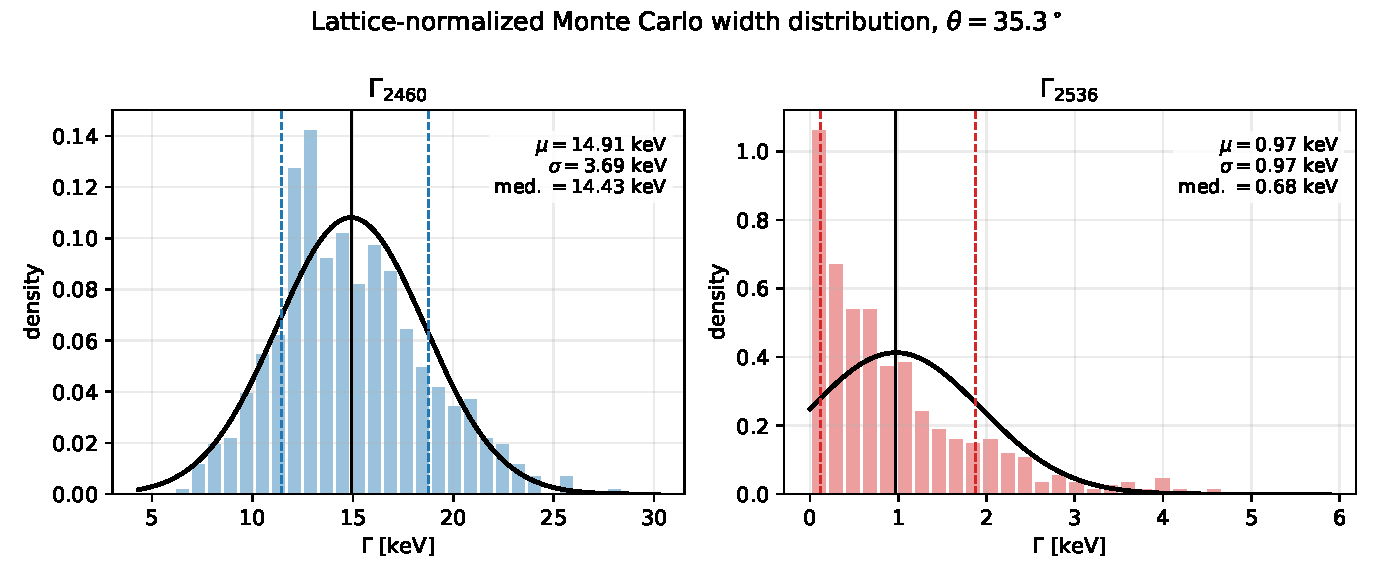
\includegraphics[width=0.47\textwidth]{../outputs/lattice_fperp_mc_width_histograms_theta_fixed.pdf}
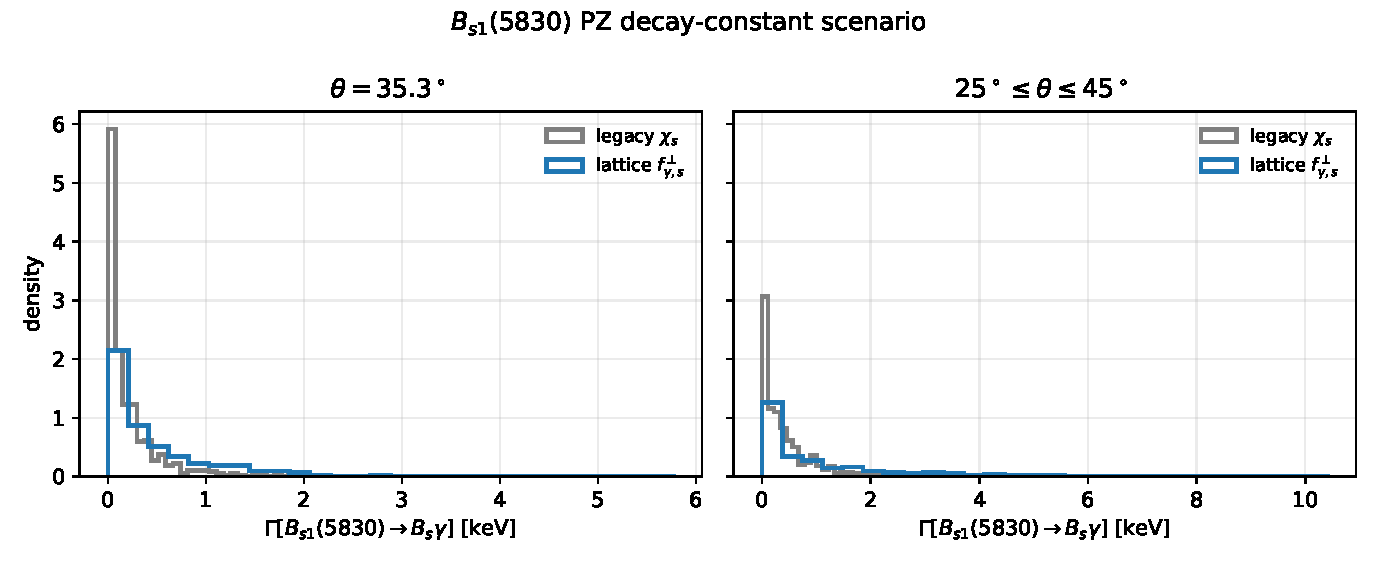
\includegraphics[width=0.47\textwidth]{../outputs/stage3_bs1_pz_width_histograms.pdf}
\caption{Monte Carlo width distributions.  Left: charm-strange
lattice-normalized photon input.  Right: bottom-strange PZ decay-constant
scenario.}
\label{fig:mc}
\end{figure}

The suppression pattern can be seen directly at the amplitude level.  With the
lattice photon normalization, the normalized pieces of the
$\Dsone(2460)$ amplitude are $-0.0715$ and $-0.205$, and therefore add
constructively.  For $\Dsone(2536)$ the corresponding pieces are $-0.0917$ and
$+0.132$, so the physical amplitude is a small difference.  This is the LCSR
counterpart of the cancellation mechanism emphasized in
Refs.~\cite{Bondar:2023mua,Bondar:2025smw}.

\subsection{Comparison with other studies and experiment}

Table~\ref{tab:literature} compares our preferred values with representative
predictions in the literature.  The comparison includes early quark-model
estimates, relativistic quark-model calculations, recent potential-model or
electric-transition analyses, and the phenomenological results of
Bondar and Milstein.  We compute the pseudoscalar final-state channels
$\Ds\gamma$ and $\Bs\gamma$.  The vector-final-state channels
$\Dst\gamma$ and $\Bst\gamma$ require separate LCSR correlators and are not
part of this paper.

\begin{table}[t]
\caption{Comparison with representative theoretical predictions.  Widths are
in keV.}
\label{tab:literature}
\begin{ruledtabular}
\begin{tabular}{lllll}
Channel & Quark models & Recent QM & Bondar--Milstein & This work\\
\hline
$\Dsone(2536)\to\Ds\gamma$ & $15$, $25.2$--$31.1$ & $18.18$--$18.85$ & $12$ & $0.504[0.127,1.104]$\\
$\Dsone(2460)\to\Ds\gamma$ & $6.2$, $10.3$--$17.2$ & $3.53$--$3.61$ & $297$ & $16.1[12.4,20.5]$\\
$\Bsone^{\rm low}(5750)\to\Bs\gamma$ & $37$, $70.6$ & $97.7$ & $47$ & $27.8[20.1,39.4]$\\
$\Bsone(5830)\to\Bs\gamma$ & $27$, $47.8$ & $56.6$ & $28$ & $0.272[0.028,1.024]$\\
\end{tabular}
\end{ruledtabular}
\end{table}

For $\Dsone(2460)$, using the measured branching fraction
$\mathcal B[\Dsone(2460)\to\Ds\gamma]=(16\pm4\pm3)\%$ \cite{BaBar:2006eep}
with our preferred partial width implies a total-width scale of order
$0.10~\MeV$, compatible with a very narrow state.  For $\Dsone(2536)$, the
measured total width $\Gamma_{\rm tot}=0.92\pm0.05~\MeV$
\cite{BaBar:2011zpy} implies a radiative branching fraction of order
$5\times10^{-4}$ in our preferred scenario.  This is far below the percent
level and naturally explains why the decay is difficult to isolate
experimentally.  For $\Bsone(5830)$ there is not yet a direct radiative
measurement, and our result should be read as a prediction for future searches.

\section{Conclusion}
\label{sec:concl}

We have calculated the radiative transitions
$\Dsone(2460)\to\Ds\gamma$, $\Dsone(2536)\to\Ds\gamma$, and
$\Bsone(5830)\to\Bs\gamma$ using light-cone QCD sum rules.  The calculation
includes hard photon emission, two- and three-particle photon DAs, and
explicit strange-quark-mass terms.  We separated the basis-current sum rules
from the physical-current residue normalization and used a lattice-normalized
photon DA as the preferred modern input.

The main result is the strong hierarchy between the two charm-strange
radiative widths.  The $\Dsone(2460)$ transition is naturally at the
tens-of-keV level, while $\Dsone(2536)\to\Ds\gamma$ is strongly suppressed by
destructive interference between the two physical-current components.  The
same cancellation-sensitive pattern appears for the observed $\Bsone(5830)$,
for which we predict a sub-keV median radiative width.

\begin{acknowledgments}
To be added.
\end{acknowledgments}

\bibliographystyle{apsrev4-2}
\bibliography{all}

\end{document}
